\chapter{Perturbation Theory}
\section{Non-Degenerate Perturbation Theory}
\subsection{General Formulation}
Suppose we have solved the time-independent Schrodinger wave equation for a given potential (in this case, an infinite potential square well)
\begin{equation}
H^0\psi_{n}^0=E^{0}_{n}\psi_{n}^0
\end{equation}
and obtaining a complete set of orthonormal eigenfunctions $\psi_{n}^0$,
\begin{equation}
\bra{\psi_{n}^0}{\psi_{m}^0}\rangle=\delta_{nm}
\end{equation}
and the corresponding eigenvalues $E^0_n$. If we perturb the potential slightly in the potential well and try to solve for the new eigenvalues and eigenfunctions, 
\begin{equation}
H\psi_n=E_n\psi_n
\end{equation}
Here, we use perturbation theory to get approximate solutions to the perturbed problem by building on the exact solutions of the unperturbed case.\\
To begin with, we write the perturbed/new Hamiltonian as the sum of two terms,
\begin{equation}
H=H^0+\lambda H'
\end{equation}
Where H' is the perturbation. We take $\lambda$ to be a small number, and the $H$ will be the true, exact Hamiltonian. Writing $\psi_n$ and $E_n$ as a power series in $\lambda$, we get,
\begin{gather}
\psi_{n}=\psi_{n}^0 + \lambda \psi_{n}^1 + \lambda^2 \psi_{n}^2+... \\
E_n= E^0_n + \lambda E^1_n + \lambda^2 E^2_n+...
\end{gather}
Here $E^1_n$ is the first-order correction to the $n^th$ eigenvalue, and $\psi_{n}^1$ is the first-order correction to the $n^th$ eigenfunction. $E^2_n$ and $\psi_{n}^2$ are the second-order corrections to the eigenvalues and eigenfunctions, and so on. Plugging in Equations (4),(5) and (6) in Equation (3) gives us,
\begin{multline}
(H^0+\lambda H')[\psi_{n}^0 + \lambda \psi_{n}^1 + \lambda^2 \psi_{n}^2+... ]=\\( E^0_n + \lambda E^1_n + \lambda^2 E^2_n+...)[\psi_{n}^0 + \lambda \psi_{n}^1 + \lambda^2 \psi_{n}^2+...]
\end{multline}
We can rewrite Equation (7) by collecting like powers of $\lambda$ in the form,
\begin{multline*}
H^0\psi^0 + \lambda(H^0\psi^1_n+H'\psi_n^0) + \lambda^2(H^0\psi^2_n+H'\psi^1_n)+...\\E^0_n\psi^0 + \lambda(E^0_n\psi^1_n+E^1_n\psi_n^0) + \lambda^2(E^0_n\psi^2_n+E_n^1\psi^1_n+E^2_n\psi^0_n)+...
\end{multline*} 
We can get the first order ($\lambda^1$) equation from Equation (7),
\begin{equation}
H^0\psi_{n}^1+H'\psi^0_n=E^0_n\psi^1_n+E^0_n+\psi_n^0
\end{equation}
And the second order ($\lambda^2$),
\begin{equation}
H^0\psi_{n}^2+H'\psi^1_n=E^0_n\psi^2_n+E^1_n\psi^1_n+E^2_n\psi^0_n
\end{equation}
And this can be done for higher powers of $\lambda$ as well.

\subsection{First order perturbation theory}
If we take the inner product of Equation (8), with $\psi^0_n$,
\begin{equation}
\langle\psi^0_n\vert H^0\psi^1_n\rangle + \langle\psi^0_n\vert H'\psi^0_n\rangle=E^0_n\langle\psi^0_n\vert\psi^1_n\rangle +E^1_0\langle\psi^0_n\vert\psi^0_n\rangle
\end{equation}
Because of the useful property of $H^0$ to be Hermitian, hence Equation (10) becomes,
\begin{equation}
\langle\psi^0_n\vert H^0\psi^1_n\rangle=\langle H^0\psi^0_n\vert \psi^1_n\rangle=E^0_n\langle\psi^0_n\vert\psi^1_n\rangle=\langle E^0_n\psi^0_n\vert\psi^1_n\rangle
\end{equation}
And hence the terms in Equation (10) cancel out and the property $\langle\psi^0_n\vert\psi^0_n\rangle=1$ give the equation,
\begin{equation}
E^1_n=\langle\psi_n^0\vert H'\vert\psi^0_n\rangle
\end{equation}
This is a fundamental result in first-order perturbation theory, and it states that first-order correction to energy is the expectation value of the pertubation in the unperturbed state.

Now to get the first-order correction to the wave function, we rewrite Equation (8),
\begin{equation}
(H^0-E^0_n)\psi^1_n=-(H'E^1_n)\psi^0_n
\end{equation}
The right side is a known fucntion, so this amounts to an inhomogenious differential equation for $\psi^!_n$. The unpertubed wave functions constitute a complete set, so $\psi^1_n$ can be writtten as a linear combination of them,
\begin{equation}
\psi^1_n=\sum_{m\neq n}c^{(n)}_m\psi^0_m
\end{equation}
We know that $\psi^0_m$ satisfies the unpertubed Schrodinger wave equation, so we have,
\begin{equation}
\sum_{m\neq n}^{}(E^0_m-E^0_n)c^{(n)}_m\psi^0_m=-(H'-E^1_n)\psi^0_n
\end{equation}

Taking the inner product with $\psi^0_l$,
\begin{equation}
\sum_{m\neg n}(E^0_m-E^0_n)c^{(n)}_m\braket{\psi^0_l}{\psi^0_m}=-\langle\psi^0_l\vert H' \vert \psi^0_n\rangle+E^1_n\braket{\psi^0_l}{\psi^0_n}
\end{equation}
If $l=n$, is zero, we then get,

\begin{equation}
E^0_m-E^0_n)c^{(n)}_l=-\langle\psi^0_l\vert H' \vert \psi^0_n\rangle
\end{equation}
Or that,
\begin{equation}
c^{(n)}_n=\frac{\langle\psi^0_m\vert H' \vert \psi^0_n\rangle}{E^0_n-E^0_m}
\end{equation}
So,
\begin{equation}
\psi^1_n=\sum_{m\neg n}\frac{\langle\psi^0_m\vert H' \vert \psi^0_n\rangle}{E^0_n-E^0_m}\psi^0_m
\end{equation}
Note that the perturbed energies are surprisingly accurate, while the wave functions are of poor accuracy.


\subsection{Second order perturbation theory}
We take the inner poduct of the second-order equation with $\psi^0_n$,
\begin{equation}
\braket{\psi^0_n}{H^0\psi^2_n}+\braket{\psi^0_n}{H'\psi^1_n}=E^0_n\braket{\psi^0_n}{\psi^2_n}+E^1_n\braket{\psi^0_n}{\psi^1_n}+ E^2_n\braket{\psi^0_n}{\psi^0_n}
\end{equation}
We exploit the Hermiticity of $H^0$,
\begin{equation}
\braket{\psi^0_n}{H^0\psi^2_n}=\braket{H^0\psi^2_n}{\psi^2_n}=E^0_n\braket{\psi^0_n}{psi^2_n}
\end{equation}
So the first term on the left cancels the first term on the right. Hence we get the formula for $E^2_n$ to be,
\begin{equation}
E^2_n=\langle\psi^0_n\vert H' \vert \psi^1_n\rangle - E^1_n\braket{\psi^0_n}{\psi^1_n}
\end{equation}
But,

\begin{equation}
\braket{\psi^0_n}{\psi^1_n}=\sum_{m\neq n}^{}c^{(n)}_m\braket{\psi^0_n}{\psi^0_m}=0
\end{equation}

so,
\begin{equation}
E^2_n=\langle\psi^0_n\vert H' \vert \psi^1_n\rangle=\sum_{m\neq n}^{}c^{(n)}_m\braket{\psi^0_n}{\psi^0_m}= \sum_{m\neq n}^{}c^{(n)}_m\frac{\langle\psi^0_m\vert H' \vert \psi^0_n\rangle \langle\psi^0_m\vert H' \vert \psi^0_n\rangle}{E^0_n-E^0_m}
\end{equation}
Therefore,
\begin{equation}
E^2_n= \sum_{m\neq n}^{}c^{(n)}_m\frac{\vert\langle\psi^0_m\vert H' \vert \psi^0_n\rangle\vert^2}{E^0_n-E^0_m}
\end{equation}
This is the fundamental result of second order perturbation theory.

\section{Degenerate Perturbation Theory}
\subsection{Motivation}
If two or more distinct states, take $\psi^0_a$ and $\psi^0_b$ share the same energy, ordinary perturbation theory fails since Equation (25) blows up. So hence we need to obtain a different way to handle the problem.

\subsection{Twofold Degeneracy}
Suppose,
\begin{align*}
H^0\psi^0_a=E^0\psi^0_a\\
H^0\psi^0_b=E^0\psi^0_b\\
\braket{\psi^0_a}{\psi^0_b=0}
\end{align*}
And note that any of linear combinations of these states,
\begin{equation}
\psi^0=\alpha\psi^0_a+\beta\psi^0_b
\end{equation}
is still an eigenstate of $H^0$, with the same eigenvalue $E^0$,
\begin{equation}
H^0\psi^0=E^0\psi^0
\end{equation}	 
When $H$ is perturbed, it breaks the degeneracy. When we increase $\lambda$, the common unperturbed energy $E^0$ splits into two. When we take away the perturbation, the upper state redyces to one linear combination of $\psi^0_a$ and $\psi^0_b$, and the lower state reduces to some other linear combination. We need to figure out the good linear combinations.\\
Now writing the good unperturbed states in general form, keeping $\alpha$ and $\beta$ adjustable and solving the Schrodinger equation,
\begin{equation}
H\psi=E\psi
\end{equation}
With $H=H^0+\lambda H'$ and,
\begin{align}
E=E^0+\lambda E^1 + \lambda^2 E^2 +...\\
\psi=\psi^0+\lambda\psi^1+\lambda^2\psi^2+...
\end{align} 
Plugging these into Equation (28) and collecting like powers of $\lambda$, as before, we find,
\begin{equation}
H^0\psi^0+\lambda(H\psi^0+H^0\psi^1)+...=E^0\psi^0+\lambda(E^1\psi^0+E^0\psi^1)+...
\end{equation}
But $H^0\psi^0=E^0\psi^0$, so the first term cancel; at order $\lambda^1$ we have,
\begin{equation}
H\psi^0+H^0\psi^1=E^1\psi^0+E^0\psi^1
\end{equation}
Taking inner product with $\psi^0_a$,
\begin{equation}
\langle\psi^0_a\vert H^0 \vert \psi^1\rangle+ \langle\psi^0_a\vert H' \vert \psi^0\rangle=E^0\braket{\psi^0_a}{\psi^1} + E^1\braket{\psi^0_a}{\psi^0}
\end{equation}
Because $H^0$ is Hermitian, the first term on the left cancels the term on the right. Putting this in Equation (26), we get,
\begin{equation}
\alpha \langle\psi^0_a\vert H' \vert \psi^0_a\rangle=\beta \langle\psi^0_a\vert H' \vert \psi^0_b\rangle=\alpha E^1
\end{equation}
Or in a more compact form,
\begin{equation}
\alpha W_{aa}+\beta W_{ab}=\alpha E^1
\end{equation}
Where,
\begin{equation*}
W_{ab}= langle\psi^0_a\vert H' \vert \psi^0_b\rangle
\end{equation*}
Similarly, the inner product with $\psi^0_b$ gives us,
\begin{equation}
\alpha W_{ba}+\beta W_{bb}=\beta E^1
\end{equation}
Now using Equation (35) and (36),
\begin{equation}
\alpha[W_{ab}W_{ba}-(E^1-W_{aa}))(E^1-W_{bb})]=0
\end{equation}
When $\alpha\neq 0$,
\begin{equation}
(E^1)^2-E^1(W_{aa}+W{bb})+(W_{aa}W_{bb}-W_{ab}W_{ba})=0
\end{equation}
Using the quadratic formula and knowing that $W_{ba}=W^*_{ab}$,
\begin{equation}
E^1_\pm=\frac{1}{2}\left[W_{aa}+W_bb\pm\sqrt{(W_{aa}-W_{bb})^2+4\vert W_{ab}\vert^2}\right]
\end{equation}
This is the fundamental result of degenerate pertubration theory, the two roots correspond to the two perturbed energies.\\
Note that when $\alpha=0$, we get the nondegenerate perturbation theory (since $\beta=1$).

\subsection{Higher-Order Degeneracy}
We start by rewriting Equations (35) and(36) in matrix form,
\begin{gather}
\begin{pmatrix}
W_{aa} & W_{ab}\\
W_{ba} & W_{bb}
\end{pmatrix}
\begin{pmatrix}
\alpha\\
\beta
\end{pmatrix}
= E^1
\begin{pmatrix}
\alpha\\
\beta
\end{pmatrix}
\end{gather}
The $E^1$s are the eigenvalues of the $W$-matrix, Equation (38) being the characteristic equation for this matrix and the good linear combinations of the unperturbed states are the eigenvectors of $W$. For $n$-fold degeneracy, we look for the eigenvalues of the $n\cross n$ matrix,
\begin{equation}
W_{ij}=\langle \psi^0_i\vert H' \vert \psi^0_j\rangle
\end{equation}
\subsection{Lamb Shift}
An interesting feature of the fine structure formula is that it depends only on $j$ and not $l$, moreover in general two different values of $l$ share the same energy. For example, the $2S_{1/2} ()$ and $2P_{1/2} ()$ states should remain perfectly degenerate. However in 1947 Lamb and Retherford performed an experiment that displayed something to the contrary. The $S$ state is slightly higher in energy than the $p$ state. The explanation of this "Lamb" shift was later explained by Bethe, Feynman, Schwinger and Tomonaga (the founders of QED) as a corollary of the electromagnetic field itself being quantised.  Sharply in contrast to the hyperfine structure of Hydrogen, the Lamb shift is a completely novel i.e. non-classical (as the hyperfine structure is explained through Coulomb's law and the Biot-Savart Law) phenomena. It arises from a radiative correction in Quantum Electrodynamics to which classical theories are mute. In Feynman lingo, this arises from loop corrections as potrayed below.
\begin{figure}[h]
	\centering
	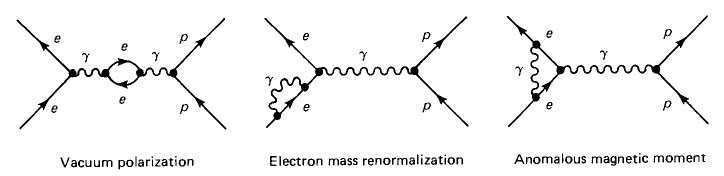
\includegraphics[width=0.6\linewidth, height=0.3\linewidth]{feyn-loop.png}
	\caption{Different kinds of radiative corrections}
\end{figure}
Naively,
\begin{enumerate}
	\item the first diagram describes pair-production in the neighbhorhood of a nucleus, leading to a partial screening effect of the proton's charge;
	\item the second diagram reflects the fact that the electromagnetic field has a non-zero ground state
	\item the third diagram leads to a tiny modification of the electron's magnetic dipole moment (an addition of $a + \alpha/2\pi = 1.00116$)
\end{enumerate}
We shall not discuss the results in depth but rather consider two exemplary cases:\\
For $ l = 0$,
\begin{equation}
\Delta E_{Lamb} = \alpha^{5}mc^{2}\frac{1}{4n^{3}}\left[k(n,0)\right]
\end{equation}
Where $k(n,0)$ is a numerical factor defined as:
$$k(n,0) = \begin{cases}
12.7, & \text{if } n = 1\\
13.2,              & \text{if } n \rightarrow \infty
\end{cases} $$
For $ l = 0$ and $j = l \pm \frac{1}{2}$,
\begin{equation}
\Delta E_{Lamb} = \alpha^{5}mc^{2}\frac{1}{4n^{3}}\left[ k(n,0) \pm \frac{1}{\pi (l + \frac{1}{2}) (l + \frac{1}{2})} \right]
\end{equation}
Here, $k(n,l)$ is a very small number $(< 0.05)$ which varies a little with it's arguments.\\
The Lamb shift is tiny except for the case $l=0$, for which it amounts to about $10 \% $ of the fine structure. However, since it depends on $l$, it lifts the degeneracy of the pairs of states with common $n$ and $j$ and in particular it splits $2 S_{1/2}$ and $2 P_{1/2}$.
\section{The Zeeman Effect}
When an atom is placed in a uniform magnetic field $B_{Ext.}$, the energy levels are shifted, this is known as the Zeeman effect. For the case of a single electron, the shift is:
\begin{equation}\label{zeeman_def}
H^{'}_{Z} = -(\mu_{l} + \mu_{s}).B_{Ext.}
\end{equation}
Where,
\begin{equation}
\mu_{s} = -\frac{e}{m_{e}}S
\end{equation}
is the magnetic dipole moment associated with electron spin, and
\begin{equation}
\mu_{l} = -\frac{e}{2m_{e}}L
\end{equation}
is the dipole moment associated with orbital motion. The gyromagnetic ratio in this case is simply classical i.e. $q/2m$, it is only for spin that we have an extra factor of 2. We now rewrite (\ref{zeeman_def}) as:
\begin{equation}
H^{'}_{Z} = \frac{e}{2m_{e}}(L + 2S).B_{Ext.}
\end{equation}
The nature of the Zeeman splitting depnds on the strength of the external field vs. the internal one that gives rise to spin-orbit/spin-spin coupling. This table provides a short review of the different cases:
\begin{center}
	\begin{tabularx}{0.9\textwidth} { 
			| >{\centering\arraybackslash}X 
			| >{\centering\arraybackslash}X 
			| >{\centering\arraybackslash}X | }
		\hline
		\textbf{Case} & \textbf{Name} & \textbf{Comments} \\
		\hline
		$B_{Ext.} >> B_{Int.}$  & Strong-Field Zeeman Effect  & Zeeman effect dominates; fine structure becomes the perturbation  \\
		\hline
		$B_{Ext.} << B_{Int.}$  & Weak-Field Zeeman Effect  & Fine structure dominates; $H^{'}_{z}$ can be treated as a small perturbation   \\
		\hline
		$B_{Ext.} = B_{Int.}$  & Intermediate Zeeman Effect  & Both the fields are equal in strength thus we would need elements of degenerate peturbation theory and will need to diagonlize the necessary portion of the Hamiltonian "by hand" \\
		\hline
	\end{tabularx}
\end{center}
In the next few sections we'll explore all of them in depth.
\subsection{Weak-Field Zeeman Effect}
Here the fine structure dominates, thus the conserved quantum numbers are $n$, $l$, $j$ and $m_{j}$, but not $m_{l}$ and $m_{s}$ due to the spin-orbit coupling L and S are not separately conserved. Generally speaking, in this problem we have a perturbation pile on top of a perturbation. Thus, the conserved quantum number are those appropriate to the dominant . In first order perturbation theory, the Zeeman correction to energy is,
\begin{equation}
E^{1}_{Z} = \expval{H^{'}_{Z}}{nlj m_{j}} = \frac{e}{2m}B_{Ext.} \expval{L + 2S}
\end{equation} 
Now to figure out $\expval{L + 2S}$, we know that $L + 2S = J + S$, this doesn't immediately tell us the expectation value of $S$ but we can figure it out as by understanding that $J = L + S$ is conserved and that the time average of $S$ is simply it's projection along $J$:
\begin{equation}
S_{Ave} = \frac{(S.J)}{J}J
\end{equation}
But, $L = J - S$, so  $L^{2} = J^{2} + S^{2} - 2 J.S$, hence:
\begin{equation}
S.J = \frac{1}{2}(J^{2} + S^{2} - 2 J.S) = \frac{\hbar^{2}}{2}[j(j+1)+ s(s+1)-l(l+1)]
\end{equation}
from which it follows that,
\begin{equation}
\expval{L + 2S} = \expval{\left(1 + \frac{S.J}{J^{2}}J\right)} = \left[1 + \frac{j(j+1)-l(l+1) + 3/4}{2j(j+1)}\right]\expval{J}
\end{equation}
The term in the square brackets is called the Lande g-factor, denoted by $g_{j}$. Now, if we choose $B_{z}$ to lie along $B_{Ext.}$, then:
\begin{equation}
E^{1}_{Z} = \mu_{B} g_{j} B_{Ext.} m_{j}
\end{equation}
where,
$$\mu_{B} = \frac{e \hbar}{2m} = 5.788 \times 10^{-5} \ eVT^{-1}$$
is the so called Bohr magneton. The total energy is the sum of the fine-structure part and the Zeeman contribution, in the ground state i.e. $n = 1, l = 0, j = 1/2$ and therefore, $g_{J} = 2$, it splits into two levels:
\begin{equation}
-13.6 \ eV(1 + \alpha^{2}/4) \pm \mu_{B} B_{Ext.}
\end{equation}
with different signs for different $m_{j}$'s this is plotted below.
\begin{figure}[h]
	\centering
	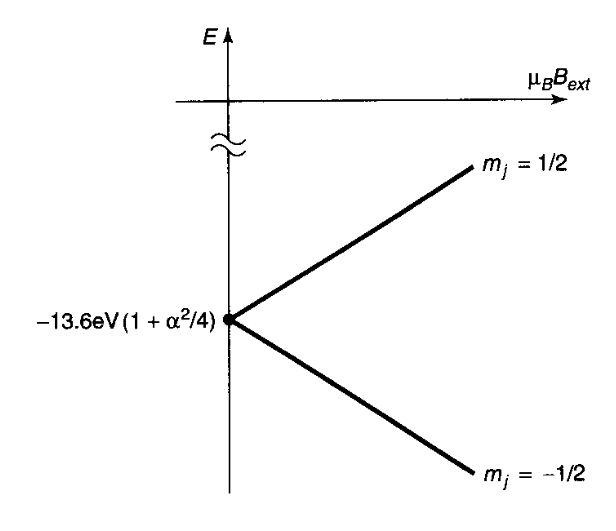
\includegraphics[width=0.6\linewidth, height=0.5\linewidth]{strong-split.png}
	\caption{Weak-field Zeeman splitting of the ground state of hydrogen; the upper line has a slope of $1$ and the lower line a slope of $-1$}
\end{figure}
\begin{figure}[h]
	\centering
	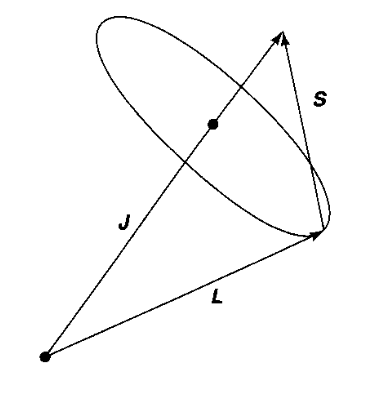
\includegraphics[width=0.6\linewidth, height=0.5\linewidth]{weak-split.png}
	\caption{In the presence of spin-orbit coupling, $L$ and $S$ are not separately conserved, they precess about the fixed total angular momentum $J$}
\end{figure}
\subsection{Strong-Field Zeeman Effect}
In this case, the Zeeman effect is often referred to as the "Paschen-Back" effect. The conserved quantum numbers are now but and because in the presence of an external torque, the total angular momentum is not conserved but the it's individual components are. The Zeeman Hamiltonian is,
\begin{equation}
H^{'}_{Z} =  \frac{e}{2m} B_{Ext.} (L_{z} + 2 S_{z})
\end{equation}
and the unperturbed energies are:
\begin{equation}
E_{nm_{l}m_{s}} = -\frac{13.6 \ eV}{n^{2}} + \mu_{B}B_{Ext.}(m_{l} + 2 m_{s})
\end{equation}
This would be our result if we ignore the fine structure completely. However, we need to take that into account as well. In first-order perturbation theory, the fine structure correction to these levels is:
\begin{equation}
E^{1}_{fs} = \expval{H^{'}_{r} + H^{'}_{so}}{n \ l \ m_{l} \ m_{s}}
\end{equation}
The relativistic contribution is the same as before for the spin-orbit term, we need
\begin{equation}
\expval{S.L} = \expval{S_{x}}\expval{L_{x}} + \expval{S_{y}}\expval{L_{y}} + \expval{S_{z}}\expval{L_{z}} = \hbar^{2}m_{l}m_{s}
\end{equation}
Here $\expval{S_{x}} = \expval{S_{y}} = \expval{L_{x}} = \expval{L_{y}} = 0$ for the eigenstates of $S_{z}$ and $L_{z}$. Putting it all together:
\begin{equation}
E^{1}_{fs} = \frac{13.6 \ eV}{n^{3}}\alpha^{2} \left(\frac{3}{4n} - \left[ \frac{l(l+1)-m_{l}m_{s}}{l(l+1/2)(l+1)}\right]\right)
\end{equation}
Th term in the square brackets is indeterminate for $l=0$, it's correct value in this case is 1. The total energy here is the sum of the Zeeman part and the fine structure contribution.
\subsection{Intermediate Zeeman Effect}
In this case, we must treat both the effects as perturbations to the Bohr Hamiltonian,
\begin{equation}
H^{'} = H^{'}_{Z} + H^{'}_{fs}
\end{equation}
In section we'll discuss the case $n = 2$, and use it as the basis for degerate perturbation theory. The states here are characterized by $l$, $j$ and $m_{j}$. We could use $l$,$m_{l}$,$m_{s}$ states but this makes the matrix elements of $H^{'}_{Z}$ easier to deal with but that of $H^{'}_{fs}$ difficult. Using the Clebsch-Gordan coefficients to express $\ket{j m_{j}}$ as a linear combination of $\ket{l m_{l}} \ket{s m_{s}}$ we have:
$$l = 0 = \begin{cases}
\psi_{1} & \ket{\frac{1}{2} \frac{1}{2}} = \ket{0 \ 0}\ket{\frac{1}{2}\frac{1}{2}}\\
\psi_{2} & \ket{\frac{1}{2} \frac{-1}{2}} = \ket{0 \ 0}\ket{\frac{1}{2}\frac{-1}{2}}
\end{cases} $$
$$l = 1 = \begin{cases}
\psi_{3} & \ket{\frac{3}{2} \frac{3}{2}} = \ket{1 \ 1}\ket{\frac{1}{2}\frac{1}{2}}\\
\psi_{4} & \ket{\frac{3}{2} \frac{-3}{2}} = \ket{1 \ -1}\ket{\frac{1}{2}\frac{-1}{2}}\\
\psi_{5} & \ket{\frac{3}{2} \frac{1}{2}} = \sqrt{2/3}\ket{1 \ 0}\ket{\frac{1}{2}\frac{1}{2}} + \sqrt{1/3}\ket{1 \ 1}\ket{\frac{1}{2}\frac{-1}{2}}\\
\psi_{6} & \ket{\frac{1}{2} \frac{1}{2}} = -\sqrt{1/3}\ket{1 \ 0}\ket{\frac{1}{2}\frac{1}{2}} + \sqrt{2/3}\ket{1 \ 1}\ket{\frac{1}{2}\frac{-1}{2}}\\
\psi_{7} & \ket{\frac{3}{2} \frac{-1}{2}} = \sqrt{1/3}\ket{1 \ -1}\ket{\frac{1}{2}\frac{1}{2}} + \sqrt{2/3}\ket{1 \ 0}\ket{\frac{1}{2}\frac{-1}{2}}\\
\psi_{8} & \ket{\frac{1}{2} \frac{-1}{2}} = -\sqrt{2/3}\ket{1 \ -1}\ket{\frac{1}{2}\frac{1}{2}} + \sqrt{1/3}\ket{1 \ 0}\ket{\frac{1}{2}\frac{-1}{2}}\\
\end{cases} $$
In this basis the matrix the non-zero elements of $H^{'}_{fs}$ are all on the diagonal and are given by the Bohr model. $H^{'}_{z}$ has four off diagonal elements. The complete matrix, W as we will see is more complicated but its eigenvalues are the same since they are independent of the chosen basis.
\begin{equation}
\begin{pmatrix}
5 \gamma - \beta & 0 & 0 & 0 & 0 & 0 & 0 & 0 \\
0 & 5 \gamma + \beta & 0 & 0 & 0 & 0 & 0 & 0\\
0 & 0 & \gamma - 2 \beta & 0 & 0 & 0 & 0 & 0\\
0 & 0 & 0 & \gamma + 2 \beta & 0 & 0 & 0 & 0\\
0 & 0 & 0 & 0 & \gamma - \frac{2}{3} \beta & \frac{\sqrt{2}}{3} \beta & 0 & 0\\
0 & 0 & 0 & 0 & \frac{\sqrt{2}}{3} \beta & 5 \gamma - \frac{1}{3} \beta & 0 & 0\\
0 & 0 & 0 & 0 & 0 & 0 & \gamma + \frac{2}{3} \beta & \frac{\sqrt{2}}{3} \beta\\
0 & 0 & 0 & 0 & 0 & 0 & \frac{\sqrt{2}}{3} \beta & 5 \gamma + \frac{1}{3} \beta
\end{pmatrix}
\end{equation}
Where,
$$\gamma = {(\alpha / 8)}^{2}13.6 \ eV$$
and,
$$\beta = \mu_{B}B_{Ext.}$$
The first four eigenvalues are already displayed along the diagonal. We only need to find the eigenvalues of the two  $2 \times 2$ blocks. The characteristic equation for the first one is given as:
\begin{equation}
\lambda^{2} - \lambda(6\gamma - \beta) + \left(5 \gamma^{2} - \frac{11}{3} \gamma \beta\right) = 0
\end{equation} 
and the quadratic formula gives the eigenvalues:
\begin{equation}
\lambda_{\pm} = 3 \gamma - (\beta /2) \pm \sqrt{4 \gamma^{2} + (2/3) \gamma \beta + (\beta^{2}/4)} 
\end{equation}
The eigenvalues of the second block are the same but with the sign of $\beta$ reversed. The eight energy levels are listed in the table and are plotted against in the figure (). In the zero field limit they reduce to the fine structure values. For the other cases, the splitting is seen clearly.
\begin{figure}[h]
	\centering
	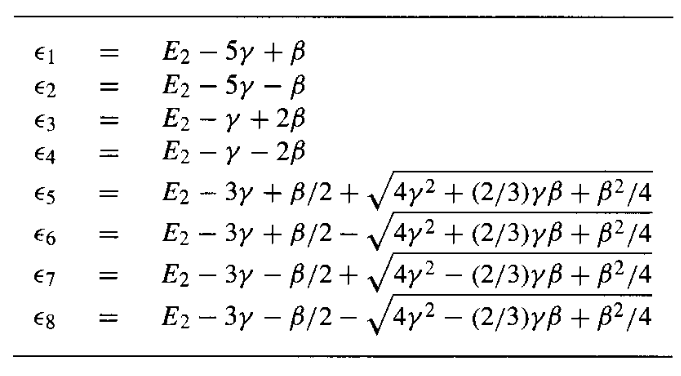
\includegraphics[width=0.6\linewidth, height=0.3\linewidth]{zee-table.png}
	\caption{Energy levels for the $n=2$ states of hydrogen, with fine structure and Zeeman splitting}
\end{figure}
\begin{figure}[h]
	\centering
	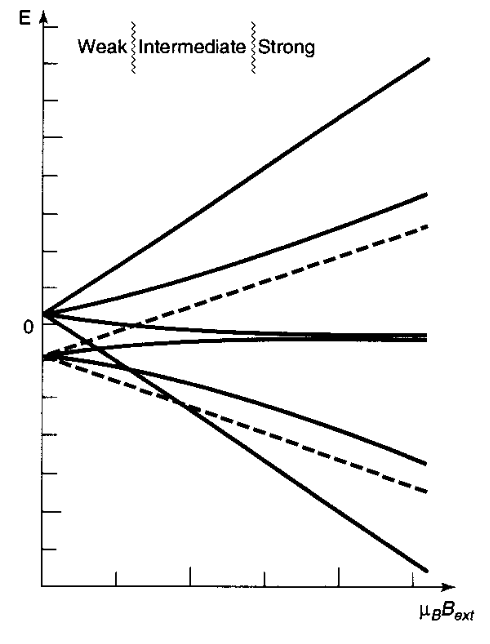
\includegraphics[width=0.6\linewidth, height=0.6\linewidth]{intermediate-split.png}
	\caption{Zeeman splitting of the $n = 2$ states of hydrogen, in the weak, intermediate and strong field regimes}
\end{figure}
\section{Hyperfine Splitting in Hydrogen}
The proton also has a magnetic dipole moment, however this is much smaller than that of the electron due to the mass of the proton. It is given by,
\begin{equation}
\mu_{p} = \frac{g_{p} e}{2 m_{p}}S_{p}
\end{equation}
And the magnetic dipole moment of the electron,
\begin{equation}
\mu_{e} = -\frac{e}{m_{e}}S_{e}
\end{equation}
Classically speaking, the dipole $\mu$ sets up a magnetic field:
\begin{equation}
B = \frac{\mu_{0}}{4 \pi r^{3}}[3(\mu . \hat{r})\hat{r} - \mu] + \frac{2 \mu_{0}}{3} \mu \delta^{3}(r)
\end{equation}
So the Hamiltonian of the electron, in the magnetic field due to the proton's magnetics dipole moment, is
\begin{equation}
H^{'}_{hf} = \frac{\mu_{0} g_{p} e^{2}}{8 \pi m_{p} m_{e}}\frac{[3(S_{p}. \hat{r})(S_{e}. \hat{r}) - S_{p}.S_{e}]}{r^{3}} + \frac{\mu_{0} g_{p} e^{2}}{3 m_{p} m_{e}}S_{p}.S_{e} \delta^{3}(r)
\end{equation}
According to perturbation theory, the first-order correcction to the energy is the expectation value of the perturbing Hamiltonian:
\begin{equation}
E^{1}_{hf} = \frac{\mu_{0} g_{p} e^{2}}{8 \pi m_{p} m_{e}} \expval{\frac{3(S_{p}.\hat{r})(S_{e}.\hat{r}) - S_{p}.S_{e}}{r^{3}}} + \frac{\mu_{0} g_{p} e^{2}}{3 m_{p} m_{e}}\expval{S_{p}.S_{e}}\abs{\psi(0)}^{2}
\end{equation}
In the groud state or any other state at which $l = 0$, the wavefunction is spherically symmetrical, and the first expectation value vanishes. Meanwhile, from the Schrodinger equation in three dimensions, we find that $\abs{\psi(0)}^{2} = 1/(\pi a^{3})$, thus,
\begin{equation}
E^{1}_{hf} = \frac{\mu_{0} g_{p} e^{2}}{3 \pi m_{p}m_{e} a^{3}}\expval{S_{p}.S_{e}}
\end{equation}
in the groud state. This is called Spin-Spin coupling because it involves the dot product of two spins in contrast with spin-orbit coupling which involves $S.L$. In the presence of spin-spin coupling, the individual spin angular momenta are no longer conserved. However the eigenvectors of the total spin is conserved:
\begin{equation}
S = S_{e} + S_{p}
\end{equation}
We square this out to get,
\begin{equation}
S_{p}. S_{e} = \frac{1}{2}(S^{2} - S^{2}_{e} - S^{2}_{p})
\end{equation}
But the electron and proton both have spin $1/2$, so $S^{2}_{e} = S^{2}_{p} = (3/4) \hbar^{2}$. In the triplet i.e. parallel spin state, the total spin is $1$, and hence $S^{2} = 2 \hbar^{2}$. In the singlet state the total spin is $0$, and  $S^{2} = 0$. Thus,
\begin{equation}
E^{1}_{hf} = \frac{4 g_{p} \hbar^{4}}{3 m_{p} m^{2}_{e}c^{2}\alpha^{4}} \begin{cases}
+1/4, & \text{ (triplet)};\\
-3/4, & \text{ (singlet)}
\end{cases}
\end{equation}
The Spin-Spin coupling breaks the spin degeneracy of the groud state, lifting the triplet and depressing the singlet, leading to an energy gap. The energy gap is given by:
\begin{equation}
\Delta E = \frac{4 g_{p} \hbar^{4}}{3 m_{p} m^{2}_{e}c^{2}\alpha^{4}} = 5.88 \times 10^{-6} \ eV
\end{equation}
\begin{figure}[h]
	\centering
	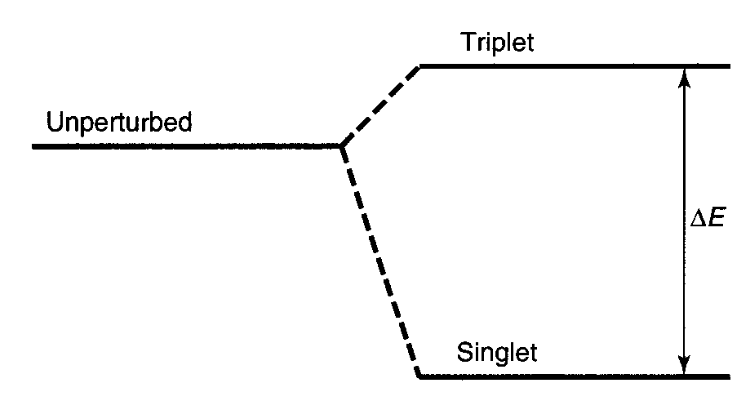
\includegraphics[width=0.6\linewidth, height=0.3\linewidth]{hyp-split.png}
	\caption{Hyperfine splitting in the ground state of Hydrogen}
\end{figure}
The frequency of the photon emitted when the triplet transitions to a singlet state is:
\begin{equation}
\nu = \frac{\Delta E}{h} = 1420 \text{ MHz}
\end{equation}
The corresponding wavelength is $21 $ cm which falls in the microwave region. It permeates the universe and is a very important part of Astrophysics.
\section{Introduction to quantum dynamics}
So far, we looked at systems that were time-independent of sorts (quantum statics), and the potentials themselves were time independent, in other words, $V(r,t)=V(r)$. Hence the time-dependent Schrodinger equation took the form,
\begin{equation}
	H\psi=i\hbar\frac{\partial \psi}{\partial t}
\end{equation}
And solving by separation of variables,
\begin{equation}
	\psi(r,t)=\psi(r)e^{iEt/\hbar}
\end{equation}
where $\psi(r)$ satisfies the time independent Schrodinger equation,
\begin{equation}
	H\psi=E\psi
\end{equation}
Due to the nature of the term that carries time dependence, the exponential factor $e^{iEt/\hbar}$, this term cancels out when we construct the physically relevant quantity $|\psi|^2$, which leads to all the expectation values and probabilities to be constant in time, and this is the same case in more complex states where we have linear combinations of these stationary states.\\
For us, if we want to investigate transitions between one energy level to another, we introduce a time-dependent potential, hence the name of quantum dynamics arises.

\section{Two level systems}
\subsection{Introduction}
Let us suppose that there are two states of the unpertubed sustem, $\psi_a$ and $\psi_b$. They are eigenstates of the unpertubed Hamiltonian, $H_0$,
\begin{align}
	H_0\psi_a=E_a  \psi_a \; \text{and} \; H_0\psi_b=E_b\psi_b
\end{align}
and they are orthonormal,
\begin{equation}
	\langle\psi_a|\psi_b\rangle=\delta_{ab}
\end{equation}
And any state can be expressed as a linear combination of them, or in particular,
\begin{equation}
	\Psi(0)=c_a\psi_a+c_b\psi_b
\end{equation}
In the absence of perturbation, each component evolves with its characteristic exponential factor.
\begin{equation}
	\Psi(t)=c_a\psi_ae^{-iE_at/\hbar}+c_b\psi_be^{-iE_bt/\hbar}
\end{equation}
Calculating $|c_a|^2$ is th probability that the particle is in he state $\psi_a$, and the measurement of the energy will yield $E_a$. Normalizing $\Psi$,
\begin{equation}
	|c_a|^2+|c_b|^2=1
\end{equation}

\subsection{The perturbed system}
Turning on a time-dependent perturbation $H'(t)$, the coefficients $c_a$ and $c_b$ become functions of $t$ and the equation then becomes,
\begin{equation}
	\Psi(t)=c_a(t)\psi_ae^{-iE_at/\hbar}+c_b(t)\psi_be^{-iE_bt/\hbar}
\end{equation} 
Now we solve for $c_a(t)$ and $c_b(t)$ by using the time-dependent Schrodinger equation,
\begin{equation}
	H\Psi=i\hbar\frac{\partial\Psi}{\partial t}, \: \text{where} \: H=H_0+H'(t)
\end{equation}

Then we see that,
\begin{equation}
	\begin{split}
		c_a[H_0\psi_a]_e^{-iE_at/\hbar}+c_b[H_0\psi_b]e^{-iE_bt/\hbar}+c_a[H'\psi_a]_e^{-iE_at/\hbar} \\
		+c_b[H'\psi_b]e^{-iE_bt/\hbar}=i\hbar[ \dot{c_a}\psi_a e^{-iE_at/\hbar}		\dot{c_b}\psi_b e^{-iE_bt/\hbar}\\
		+c_a\psi_a\left(\frac{iE_a}{\hbar}\right)  e^{-iE_at/\hbar}+ c_b\psi_b\left(\frac{iE_b}{\hbar}\right)  e^{-iE_bt/\hbar}]
	\end{split}
\end{equation}
This then simplifies to,
\begin{equation}
	c_a[H'\psi_a]_e^{-iE_at/\hbar}+c_b[H'\psi_b]e^{-iE_bt/\hbar}=i\hbar[ \dot{c_a}\psi_a e^{-iE_at/\hbar}		\dot{c_b}\psi_b e^{-iE_bt/\hbar}
\end{equation}
We isolate $\dot{c_a}$ by taking the inner product with $\psi_a$ and exploiting the orthogonality of $\psi_a$ and $\psi_b$.
\begin{equation}
	c_a\langle \psi_a| H'|\psi_a\rangle_e^{-iE_at/\hbar}+c_b\langle \psi_a|H'|\psi_b]e^{-iE_bt/\hbar}=i\hbar\dot{c_a}e^{-iE_at/\hbar}
\end{equation}
Then we define,
\begin{equation}
	H'_{ij}\equiv\langle\psi_i|H'|\psi_j\rangle
\end{equation}
The hermiticity of $H'$ says that $H'_{ji}=(H'_ij)^*$. Now multiplying with $-(i/\hbar)e^{iE_at/\hbar}$, we conclude that,
\begin{equation}
	\dot{c_a}=-\frac{i}{\hbar}[c_aH'_{aa}+c_bH'_{ab}e^{-i(En-E_a)t/\hbar}]
\end{equation}
Similarly the inner product with $\psi_b$ isolate $\dot{c_b}$ and gives the result,

\begin{equation}
	\dot{c_b}=\frac{i}{\hbar}[c_bH'_{bb}+c_aH'_{ba }e^{-i(En-E_a)t/\hbar}]
\end{equation}
Equations (15) and (16) are equivalent to the time-dependent Schrodinger equation for a two level system. And the diagonal matrix elements of $H'$ vanish giving,
\begin{equation}
	H'_{aa}=H'_{bb}=0
\end{equation}
And the equations simplify to,
\begin{align}
	\dot{c_a}=-\frac{i}{\hbar}H'_{ab}e^{-i\omega_0t}c_b \\
	\dot{c_b}=-\frac{i}{\hbar}H'_{ab}e^{i\omega_0t}c_a
\end{align}
Where,
\begin{equation*}
	\omega_0=\frac{E_b-E_a}{\hbar}
\end{equation*}

\subsection{Time-Dependent Perturbation Theory}
Defining a size for the perturbation $H'$, considering it to be small, we can obtain solutions for equations (18) and (19) by the process of successive approximations.\\
Suppoe the particle starts out in the lower state,
\begin{equation}
	c_a(0)=1. \; c_b(0)=0
\end{equation}
If there exists no perturbation, these states remain iike this forever.\\

\textbf{Zeroth Order:} \\
\begin{equation}
	c^{(0)}_a(t)=1 \; c^{(0)}_b(t)=0
\end{equation}
To calculate the first-order approximation, we insert these values on the right side of equations (18) and (19)\\
\\
\textbf{First Order:} \\
\begin{equation*}
	\frac{dc_a}{dt}=0 \rightarrow c^{(1)}_a(t)=1;
\end{equation*}	
\begin{equation}
	\frac{dc_b}{dt}=-\frac{i}{\hbar}H'_{ba}e^{i\omega_0t}\rightarrow c^{(1)}_b=\frac{i}{\hbar}\int_{0}^{t}H'_{ba}(t')e^{i\omega_0t'}dt'
\end{equation}
\\
\textbf{Second Order:}\\
\begin{equation*}
	\frac{dc_a}{dt}=-\frac{i}{\hbar}H'_{ba}e^{i\omega_0t}\left(\frac{i}{\hbar}\right)\int_{0}^{t}H'_{ba}(t')e^{i\omega_0t'}dt'\rightarrow
\end{equation*}
\begin{equation}
	c^{(2)}_a(t)=1-\frac{1}{\hbar}\int_{0}^{t}H'_{ab}(t')e^{i\omega_0t'}\left[\int_{0}^{t'}H'_{ba}(t'')e^{i\omega_0t''}dt''\right]dt'
\end{equation}
We can continue this process for obtaining n-order approximations.

\subsection{Sinusoidal Perturbations}
If the perturbation has sinusoida time dependence,
\begin{equation}
	H'(r,t)=V(r)cos(\omega t)
\end{equation}
so that,
\begin{equation}
	H'_{ab}=V_{ab}cos(\omega t)
\end{equation}
Where,
\begin{equation}
	V_{ab)}\equiv \langle\psi_a|V|\psi_b\rangle
\end{equation}
For the first order perturbations, using equation (22),
\begin{equation}
	c_b(t)\approx -\frac{i}{\hbar}\int_{0}^{t}cos(\omega t')dt'=-\frac{iV_ba}{2\hbar}\int_{0}^{t}\left[e^{i(\omega_0+\omega)t'}+e^{i(\omega_0-\omega)t'}\right]dt'
\end{equation}
\begin{equation}
	=-\frac{V_{ba}}{2\hbar}\left[\frac{e^{i(\omega_0+\omega)t}-1}{\omega_0+\omega}	+ \frac{e^{i(\omega_0-\omega)t}-1}{\omega_0-\omega}	\right]
\end{equation}
Simplifying this equation by restricting our attention to driving frequency $\omega$ close to transition frequence $\omega_0$, the second term dominates. To be more specific, we assume,
\begin{equation}
	\omega_0+\omega>>|\omega_0-\omega|
\end{equation}
Perturbation at other frequencies have negligible probabilty for causing a transistion, so this isnt a limitation. Now the equation simplifies to,
\begin{equation*}
	c_b(t)\approx-\frac{V_{ba}}{2\hbar} \frac{e^{i(\omega_0-\omega)t}-1}{\omega_0-\omega}[e^{i(\omega_0-\omega)t/2}-e^{-i(\omega_0-\omega)t/2}]
\end{equation*}
\begin{equation}
	=-i\frac{V_{ba}}{\hbar}\frac{sin[(\omega_0-\omega) t/2]}{\omega_0-\omega}e^{i(\omega_0-\omega)t/2}
\end{equation}

The transition probability, the probability that a particle which started out in the state $ \psi_a $ wil be found at a time $t$, in the state $\psi_b$ is,
\begin{equation}
	P_{a\rightarrow b}(t)=|c_b(t)^2\approx \frac{|V_{ba}|^2}{\hbar^2}\frac{sin^2[(\omega_0-\omega) t/2]}{(\omega_0-\omega)^2}
\end{equation}	

\section{Emission and Absorption of Radiation}
\subsection{Electromagnetic Waves}
An atom, in the presence of a passing light wave, responds to the electric component. It is sinusoidal in nature,
\begin{equation}
	E= E_0cos(\omega t)\hat{k}
\end{equation}
Where $q$ is the charge of the electron. Evidently,
\begin{equation}
	H'_{ba}=-\wp E_0cos(\omega t), \; \wp\equiv q\langle\psi_b|z|\psi_a\rangle
\end{equation}
When $\psi$ is an even or odd function of $z$, $z|\psi|^2$ is odd and integrates to zero, hence the diagonal matrix elements of $H'$ vanish, hence the perturbation is oscillatory and is of the form,
\begin{equation}
	V_{ba}=-\wp E_0
\end{equation}

\subsection{Absorption, stimulated emission and spontaneous emission}
If an atom starts in the lower state $\psi_a$ and you shine a polarized moochromatic beam of light on it, the probablilty of a transistion to the "upper" state $\psi_b$ is given by,
\begin{equation}
	P_{a\rightarrow b}(t)=\left(\frac{\wp E_0}{\hbar}\right)^2\frac{sin^2[(\omega_0-\omega) t/2]}{(\omega_0-\omega)^2}
\end{equation}
The atom absorbs an energy of $E_B-E_a=\hbar\omega_0$ from the electromagnetic field. We could say that it has absorbed a photon.\\
Now doing the same derivation for the transition from lower to upper state, we get
\begin{equation}
	P_{b\rightarrow a}(t)=\left(\frac{\wp E_0}{\hbar}\right)^2\frac{sin^2[(\omega_0-\omega) t/2]}{(\omega_0-\omega)^2}
\end{equation}
Here we note that the probability of transition from $a\rightarrow b$ is the same as $b\rightarrow a$, and this was called stimulated emission. The electromagnetic field gains energy $\hbar\omega_0$ from the atom.\\
Spontaneous emission is when an atom in the excited state makes a transition downward with a release of a photon without the application of any electromagnetic field.

\subsection{Incoherent perturbations}
The energy density of an electromagnetic wave is,
\begin{equation}
	u=\frac{\epsilon_0}{2}E^2_0
\end{equation}	
The transition probablity is proportional to the energy density of the fields,
\begin{equation}
	P_{b\rightarrow a}(t)=\frac{2u}{\epsilon_0\hbar^2}|\wp|^2\frac{sin^2[(\omega_0-\omega) t/2]}{(\omega_0-\omega)^2}
\end{equation}
But this is for a monochromatic perturbation for a single frequency $\omega$, now subjecting the system to a range of frequencies, $u\rightarrow\rho(\omega)d\omega$ where $\rho(\omega)d\omega$ is the enegy density in the frequency range $d\omega$ and the net transistion probability takes the form of an integral,
\begin{equation}
	P_{b\rightarrow a}(t)=\frac{2}{\epsilon_0\hbar^2}|\wp|^2 \int_{0}^{\infty}\rho(\omega)\left\{\frac{sin^2[(\omega_0-\omega) t/2]}{(\omega_0-\omega)^2}\right\}d\omega
\end{equation}	
The term in the curly brakets is sharply peaked about $\omega_0$. while $\rho(\omega)$ is relatively broad, so we replace $\rho(\omega)$ with $\rho(\omega_0)$ anf tak it outside the integral,
\begin{equation}
	P_{b\rightarrow a}(t)\approx\frac{2|\wp|^2}{\epsilon_0\hbar^2}\rho(\omega_0)\ \int_{0}^{\infty}\left\{\frac{sin^2[(\omega_0-\omega) t/2]}{(\omega_0-\omega)^2}\right\}d\omega
\end{equation}
Changing variables from $x\equiv(\omega_0-\omega)t/2$, extending the limits of integration to $x=+_-\infty$, looking up the definite integral,
\begin{equation*}
	\int_{-\infty}^{\infty}\frac{sin^2x}{x^2}dx=\pi
\end{equation*}
we find that,
\begin{equation}
	P_{b\rightarrow a}(t)\approx\frac{\pi|\wp|^2}{\epsilon_0\hbar^2}\rho(\omega_0)t
\end{equation}	
The transition probability is proportional to $t$. The flopping phenomenon characteristic of a monochromatic perturbation gets washed out when we hit the system with an incoherent spread of frequencies. The transition rate 
is now a constant,
\begin{equation}
	R_{b\rightarrow a}=\frac{\pi}{\epsilon_0\hbar}|\wp|^2\rho(\omega_0)
\end{equation}	
We take all possible polarisations and not only from x and z directions, hence instead of $|\wp|^2$, we have an average $|\hat{n}\cdot\bm{\wp}|^2$, where
\begin{equation}
	\bm{\wp}=q\langle\psi_b|r|\psi_a\rangle
\end{equation}	
And the average is over both polarisations and over all incident directions. This averaging is carried out as follows,\\
\\
\textbf{Polarisation:} For propogation in the z-direction, the two possible polarisations are $\hat{i}$ and $\hat{j}$, so the polarisation average ($p$) is,
\begin{equation}
	(\hat{n}\cdot\bm{\wp})^2_p=\frac{1}{2}[	(\hat{i}\cdot\bm{\wp})^2+ 	(\hat{j}\cdot\bm{\wp}^2)=\frac{1}{2}\wp^2 sin^2\theta 
\end{equation}
Where $\theta$ is the angle between $\bm{\wp}$ and the direction of propogation.\\
\\
\textbf{Propogation direction}:	Setting the polar axis along $\bm{\wp}$ and integrate over all propogation directions to get the polarisation-propogation average,

\begin{equation}
	(\hat{n}\cdot\bm{\wp})^2_pp=\frac{1}{4\pi}\int\left[\frac{1}{2}\wp^2 \sin^2\theta\right]sin\theta d\theta d\phi=\frac{\wp^2}{4}\int_{0}^{\pi}\sin^3\theta d\theta=\frac{\wp^3}{3} 
\end{equation}
So the transition rate for the stimulated emission from state $b$ to state $a$, under the influence of incoherent, unpolarized light incident from all directions, is,
\begin{equation}
	R_{b\rightarrow a}=\frac{\pi}{3\epsilon_0\hbar^2}|\bm{\wp}|^2\rho(\omega_0)
\end{equation}
Where \bm{$\wp$} is the matrix element of the electric dipole moment between the two tate and $\rho(\omega_0)$ is the energy density in the fields, per unit frequency, evaluated at $\omega_0=(E_b-E_a)/\hbar$.

\section{Spontaneous Emission}
\subsection{Einstein's A and B coefficients}
Picture a container of atoms, $N_a$ of them in a lower state $\psi_a$ and $N_b$ of them in the upper state $\psi_b$. Let A be the spontaneous emission rate, so that the number of particle leaving the upper state by this process per unit time is $N_bA$. The transition rate for stimulated emission is proportional to the energy density of the electromagnetic field. The number of upper state particles leaving is also similarly found. The absorption rate is proportional to $\rho(\omega_0)$. Now,
\begin{equation}
	\frac{dN_b}{dt}=-N_bA-N_bB_{ba}\rho(\omega_0)+N_aB_{ab}\rho(\omega_0)
\end{equation}
Supposing that the atoms are in thermal equlibrium with the ambient field so that the number of particles in each level is constant. $dN_b/dt=0$, hence,
\begin{equation}
	\rho(\omega_0)=\frac{A}{(N_a/N_b)B_{ab}-B_{ba}}
\end{equation}

From statistical mechanics, the number of particles with energy $E$. in thermal equilibrium at temperature $T$, is proportional to the Boltzmann factor, $e^{-E/k_bT}$, so
\begin{equation}
	\frac{N_a}{N_b}=\frac{e^{-E_a/k_bT}}{e^{E_b/k_bT}}=e^{\hbar\omega_0/k_bT}
\end{equation}
and hence,
\begin{equation}
	\rho(\omega_0)=\frac{A}{e^{\hbar\omega_0/k_bT}}B_{ab}-B_{ba}
\end{equation}
From Planck's blackbody formula,
\begin{equation}
	\rho(\omega)=\frac{\hbar}{\pi^2c^3}\frac{\omega^3}{e^{\hbar\omega/k_bT}-1}
\end{equation}
And from these two equations we can deduce that,
\begin{equation}
	B_{ab}=B_{ba}
\end{equation}
And so,
\begin{equation}
	A=\frac{\omega^3\hbar}{\pi^2c^3}B_{ba}
\end{equation}
We see that from equation (52), that the transition rate for stimulated emission is the same as for absorption. Now, we deduce from equation (46) that,
\begin{equation}
	B_{ba}= frac{\pi}{3\epsilon_0\hbar^2}|\bm{\wp}|^2
\end{equation}
And spontaneous emission rate is,
\begin{equation}
	A=\frac{\omega^3|\bm{\wp}|^2}{3\pi\epsilon_0\hbar c^3}
\end{equation}

\subsection{The lifetime of an excited state}
Suppose that you have a bottle full of atoms, with $B_b(t)$ of them in the excited stat. Due to spontaneous emission, this number decreases as time goes on, and to be more specifi, in a time interval $dt$ you will lose a fraction of $Adt$ of them,
\begin{equation}
	dN_b=-AN_bdt
\end{equation}	
Solving for $N_b(t)$, we get,
\begin{equation}
	N_B(t)=N_b(0)e^{-At}
\end{equation}
Here we can see that the number remaining in the excited state decreases exponentially, with a time constant,
\begin{equation}
	\tau=\frac{1}{A}
\end{equation}
We call this the lifetime of a state, or to be more technical, it is the time taken for $N_B(t)$ to reach $1/e\approx0.368$ of its initial value.\\
Suppose that there are many more states, and many more decays, the transition rates add up, and the net lifetime is,
\begin{equation}
	\tau=\frac{1}{A_1+A_2+A_3+...}
\end{equation}

\subsection{Selection rules}
The calculation of spontaneous emission rates are reduced to a matter of evaluating matrix elements of the form,
\begin{equation*}
	\langle\psi_b|\textbf{r}|\psi_a\rangle
\end{equation*}
Specifying the states with quantum numbers $n$, $l$ and $m$,	
\begin{equation}
	\langle b'l'm'|\textbf{r}|nlm\rangle
\end{equation}
Exploitatio of the angular momentum commutation relations and the hermiticity of the angular momentum operators yield these constraints on this quantity,\\
\\
\textbf{Selection rules involving $m$ and $m'$:} No transitions occur unless $\Delta m=+_-1$ or $0$\\
\\
\textbf{Selection rules involving $l$ and $l'$:} No transitions occur unless $\Delta l=+_-1$










